\documentclass{../presentation}

\begin{document}

\frame[plain]{\titlepage}

\begin{frame}{Aufgaben}
    \begin{itemize}
        \item Aufräumen
        \item Model/MDH/TPS überführen
    \end{itemize}
\end{frame}

\begin{frame}{Status: Visualizer}
    \begin{itemize}
        \item Alter Kode wurde entfernt
    \end{itemize}
\end{frame}

\begin{frame}{Status: MDH2Vis}
    \begin{itemize}
        \item Erzeugt eine Konfiguration
        \item Leicht erweiterbar
        \item Kamera muss überarbeitet werden
    \end{itemize}
\end{frame}

\begin{frame}{Ausgabe}
    \begin{center}
        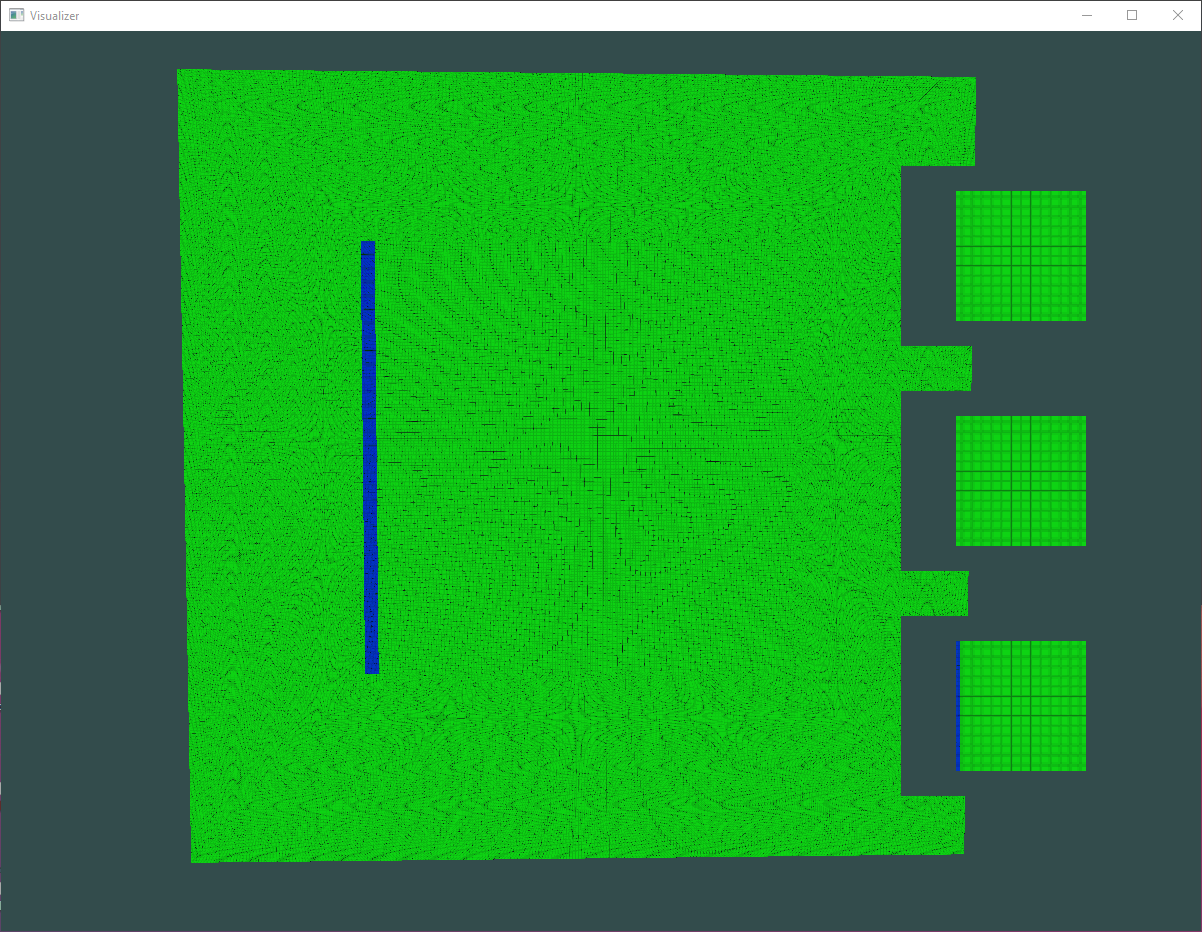
\includegraphics[width=0.8\textwidth]{visualizer_output.png}
    \end{center}
\end{frame}

\begin{frame}{Schwierigkeiten}
    \begin{itemize}
        \item Artefakte an der Textur
        \item Ziemlich klein
    \end{itemize}
\end{frame}

\begin{frame}{Tool}
    \begin{itemize}
        \item NVIDIA Nsight Graphics
        \item Ähnelt einem Debugger für die GPU
        \item Zeigt alle Ressourcen und Ausgaben an
    \end{itemize}
\end{frame}

\begin{frame}{View 1}
    \begin{center}
        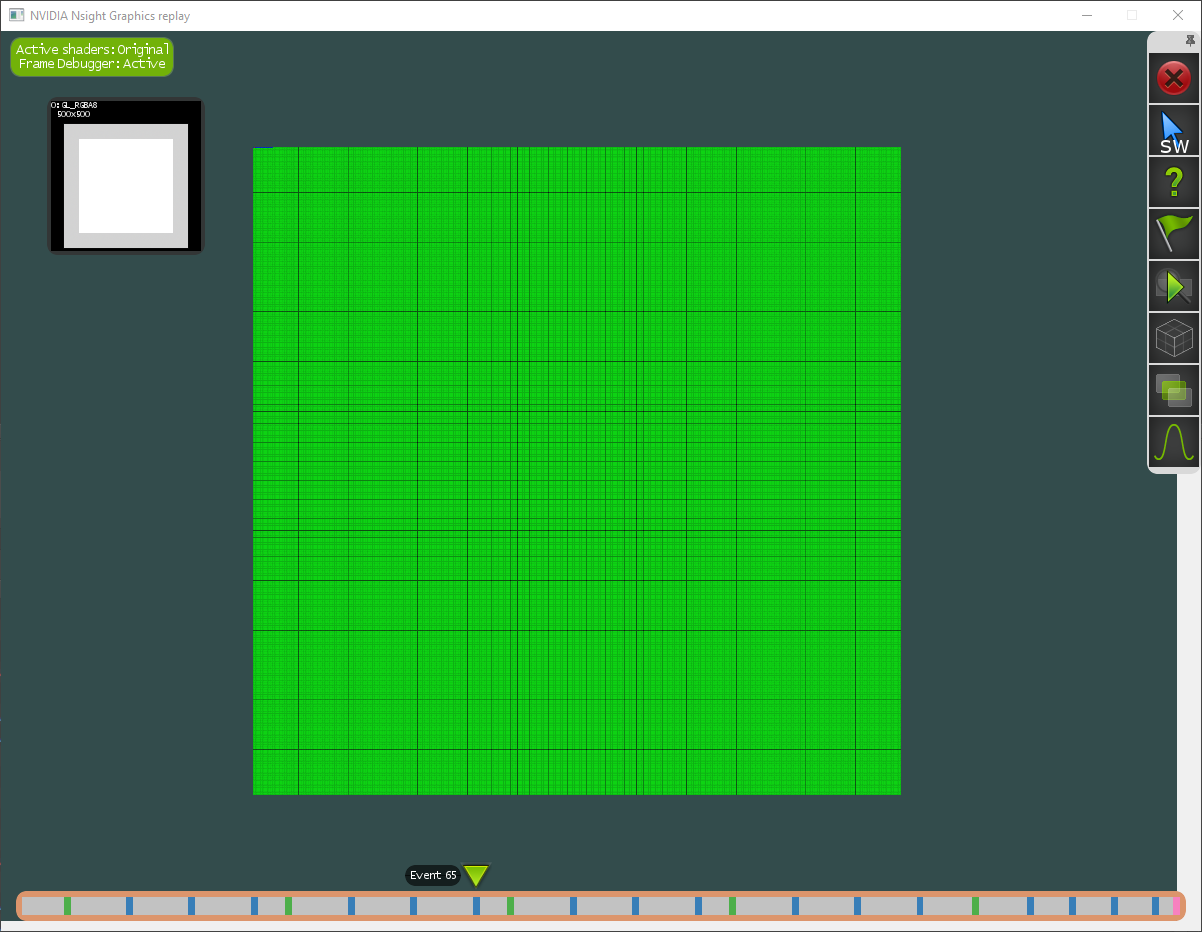
\includegraphics[width=0.8\textwidth]{visualizer_1_full.png}
    \end{center}
\end{frame}

\begin{frame}{View 1}
    \begin{center}
        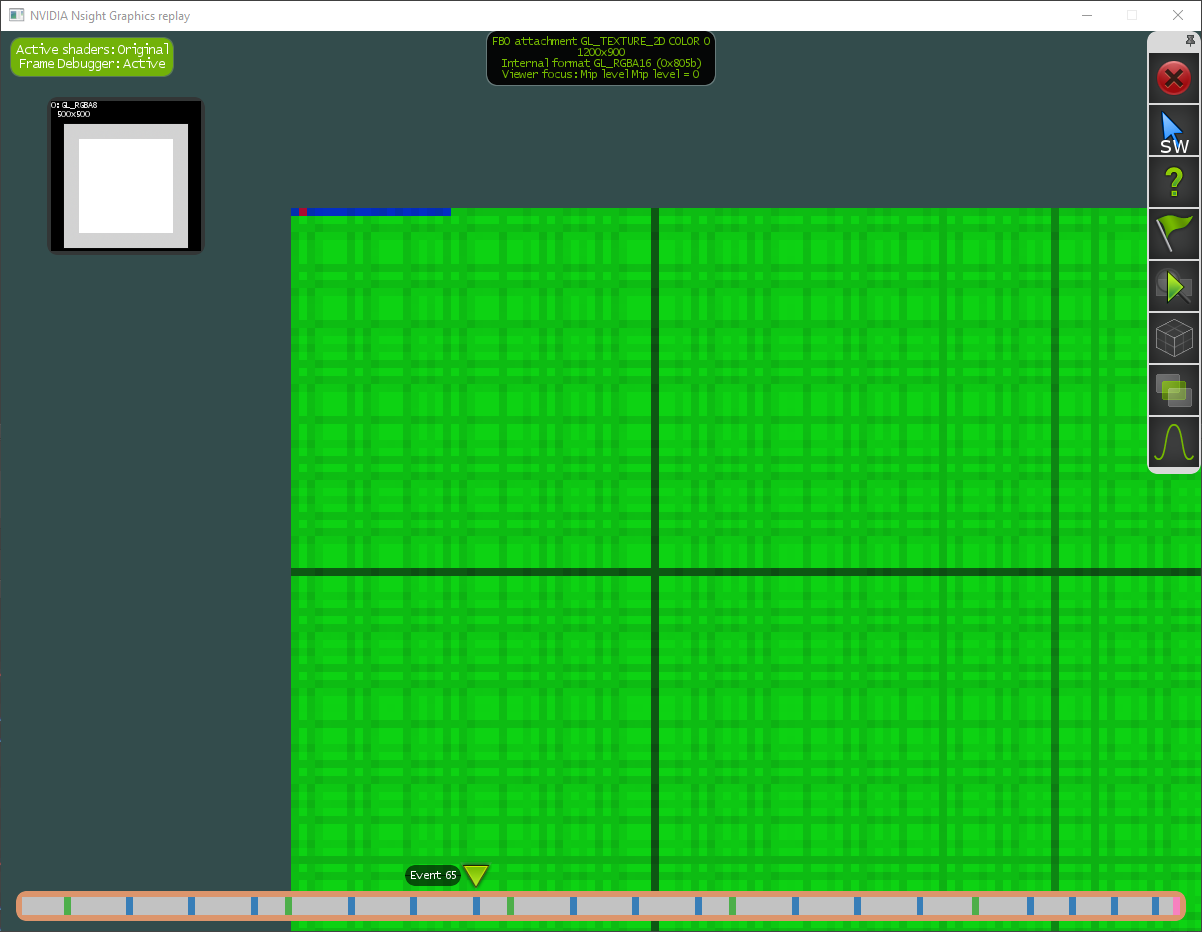
\includegraphics[width=0.8\textwidth]{visualizer_1_zoom.png}
    \end{center}
\end{frame}

\begin{frame}{View 2}
    \begin{center}
        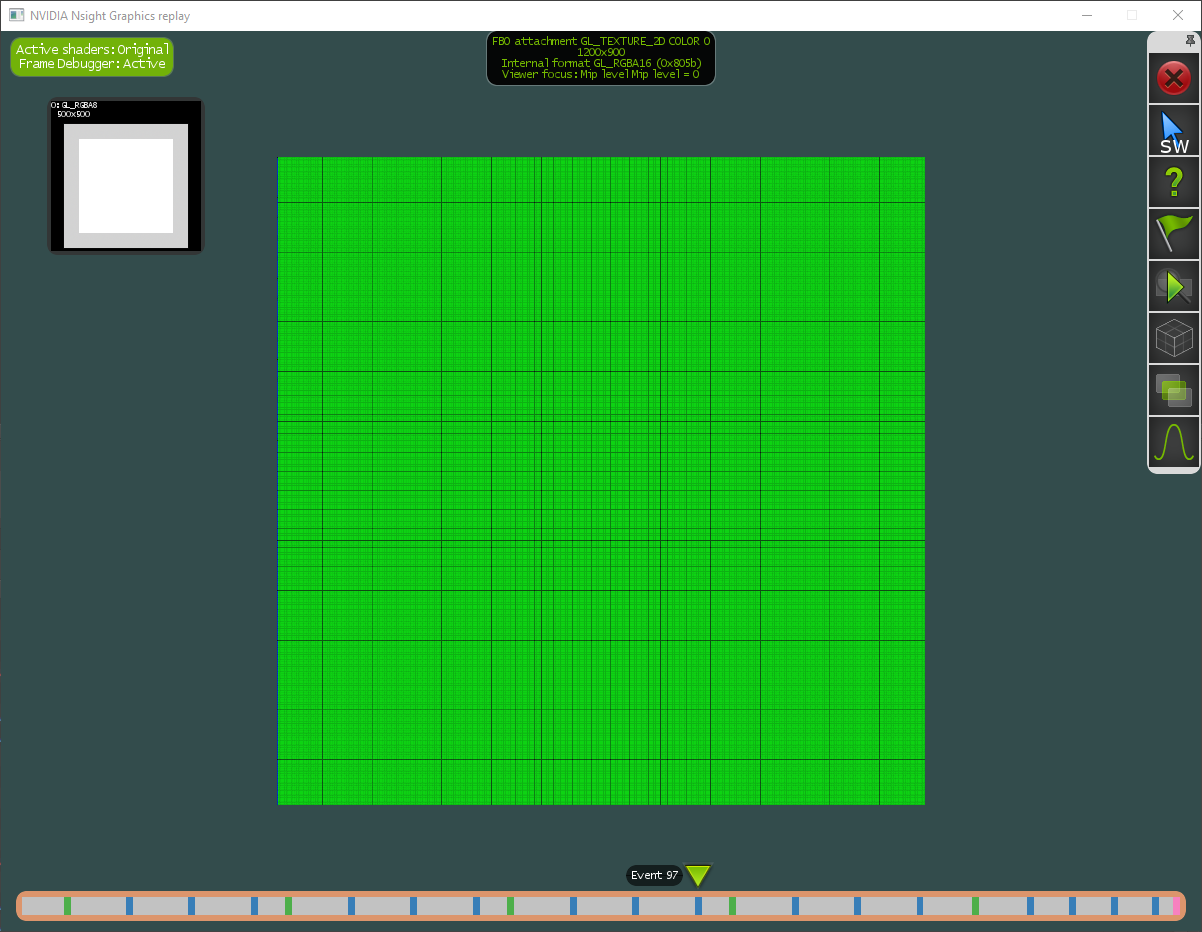
\includegraphics[width=0.8\textwidth]{visualizer_2_full.png}
    \end{center}
\end{frame}

\begin{frame}{View 2}
    \begin{center}
        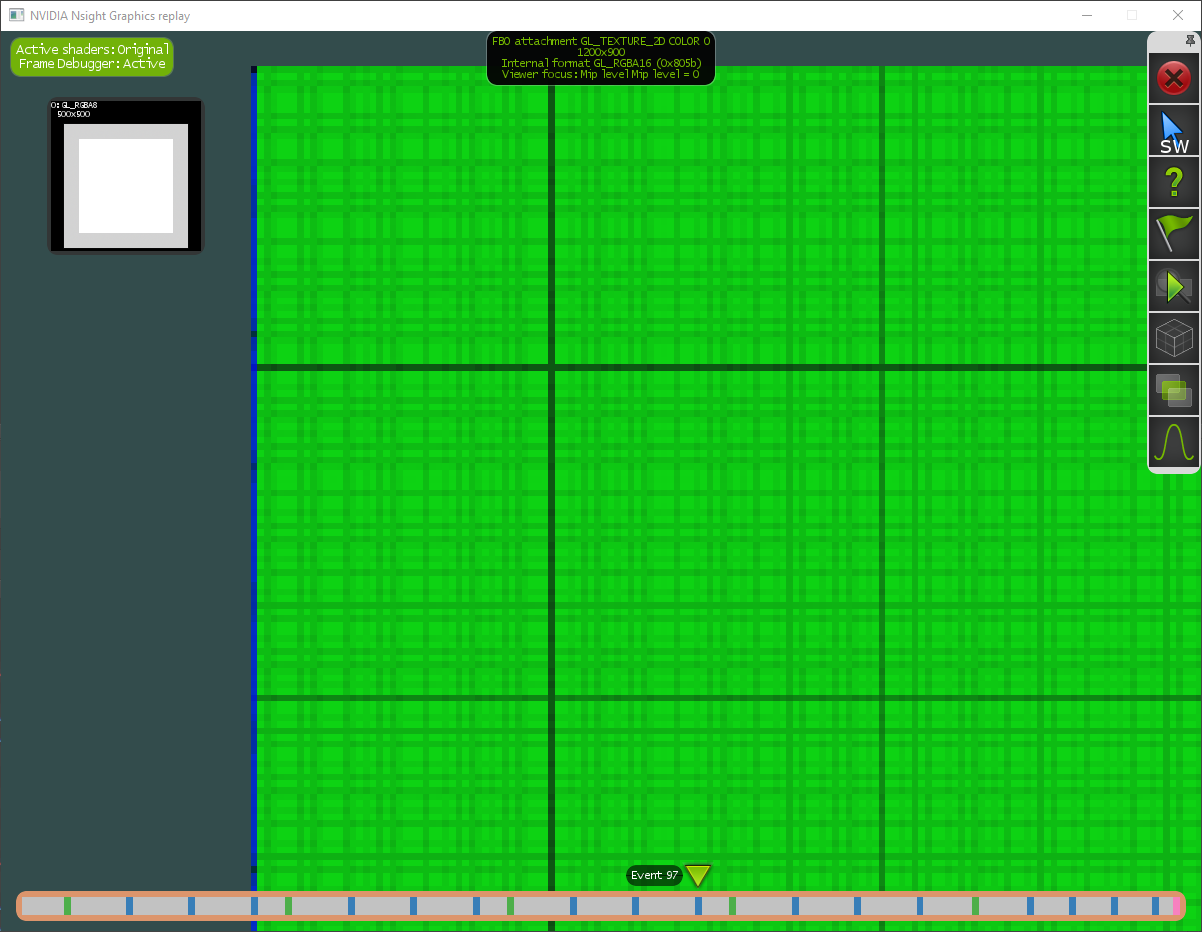
\includegraphics[width=0.8\textwidth]{visualizer_2_zoom.png}
    \end{center}
\end{frame}

\begin{frame}{View 3}
    \begin{center}
        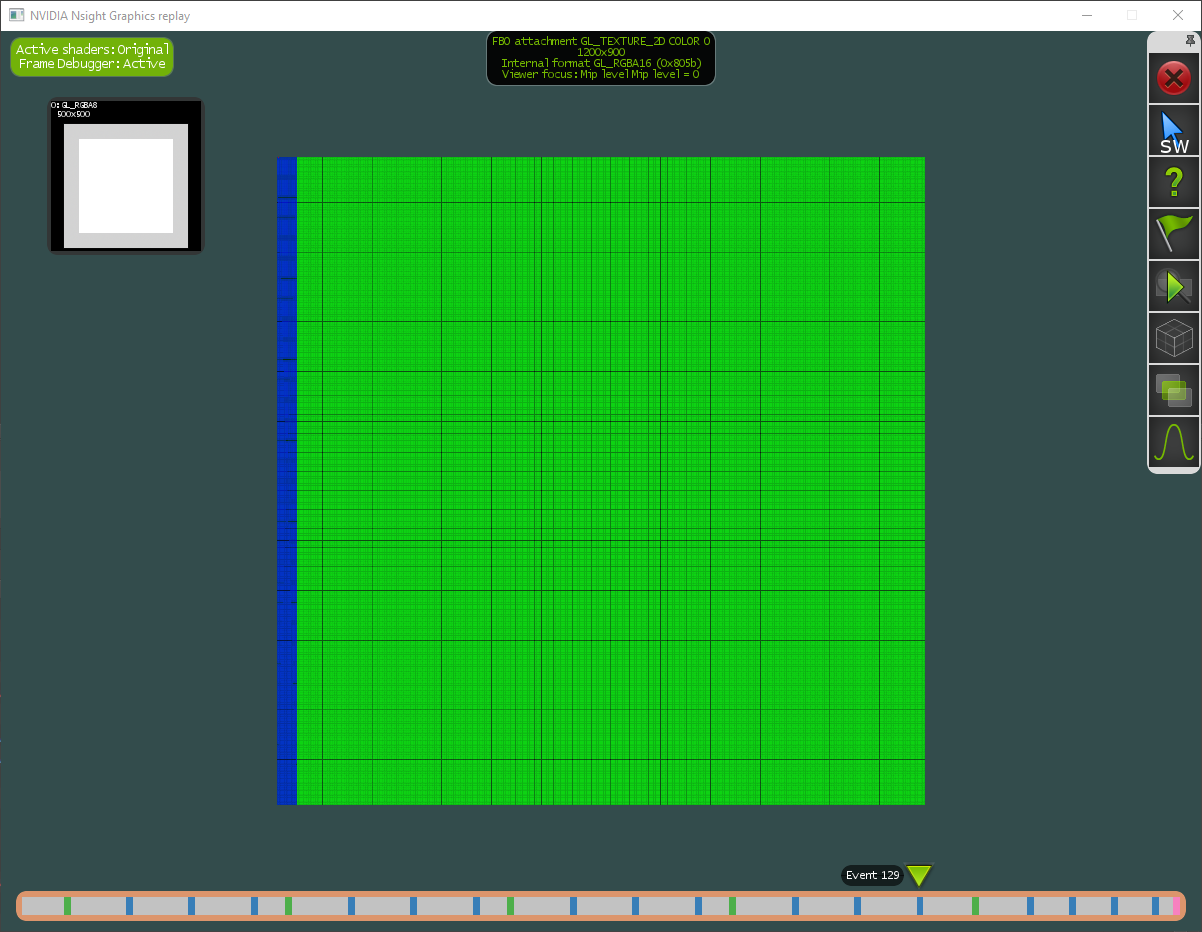
\includegraphics[width=0.8\textwidth]{visualizer_3_full.png}
    \end{center}
\end{frame}

\begin{frame}{View 3}
    \begin{center}
        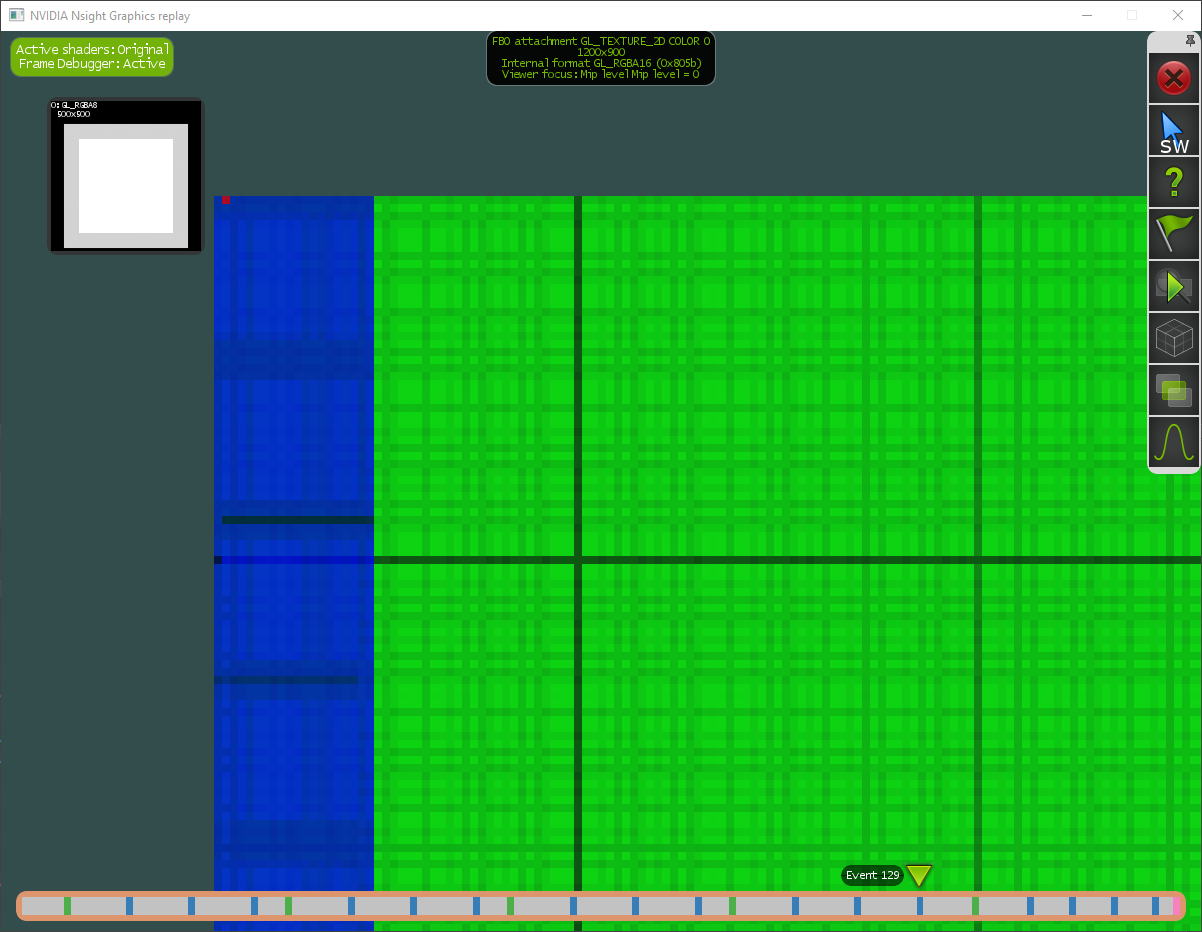
\includegraphics[width=0.8\textwidth]{visualizer_3_zoom.png}
    \end{center}
\end{frame}

\begin{frame}{Aufgaben}
    \begin{itemize}
        \item Fehler beheben
        \item Bessere Kamera implementieren
        \item MDH2Vis erweitern
    \end{itemize}
\end{frame}


\end{document}

% vi: tw=100
